%---------------------------------
\vspace{-0.6em}
\section{Method}
\label{sec:method}
%---------------------------------

We propose a method to equip pre-trained Text-to-Video (T2V) models with a style adapter, allowing for the generation of stylized videos based on both a text prompt and a style reference image. The overview is illustrated in Figure~\ref{fig:overview}. In this framework, the textual description dictates the video content, while the style image governs the visual style, ensuring a disentangled control over the video generation process.
Given the limited availability of stylized videos, we employ a two-stage training strategy. Initially, we utilize an image dataset abundant in artistic styles to learn reference-based style modulation. Subsequently, adaptation finetuning on a mixed dataset of style images and realistic videos is conducted to improve the temporal quality of the generated videos.


%
\begin{figure}[t]
    \centering
    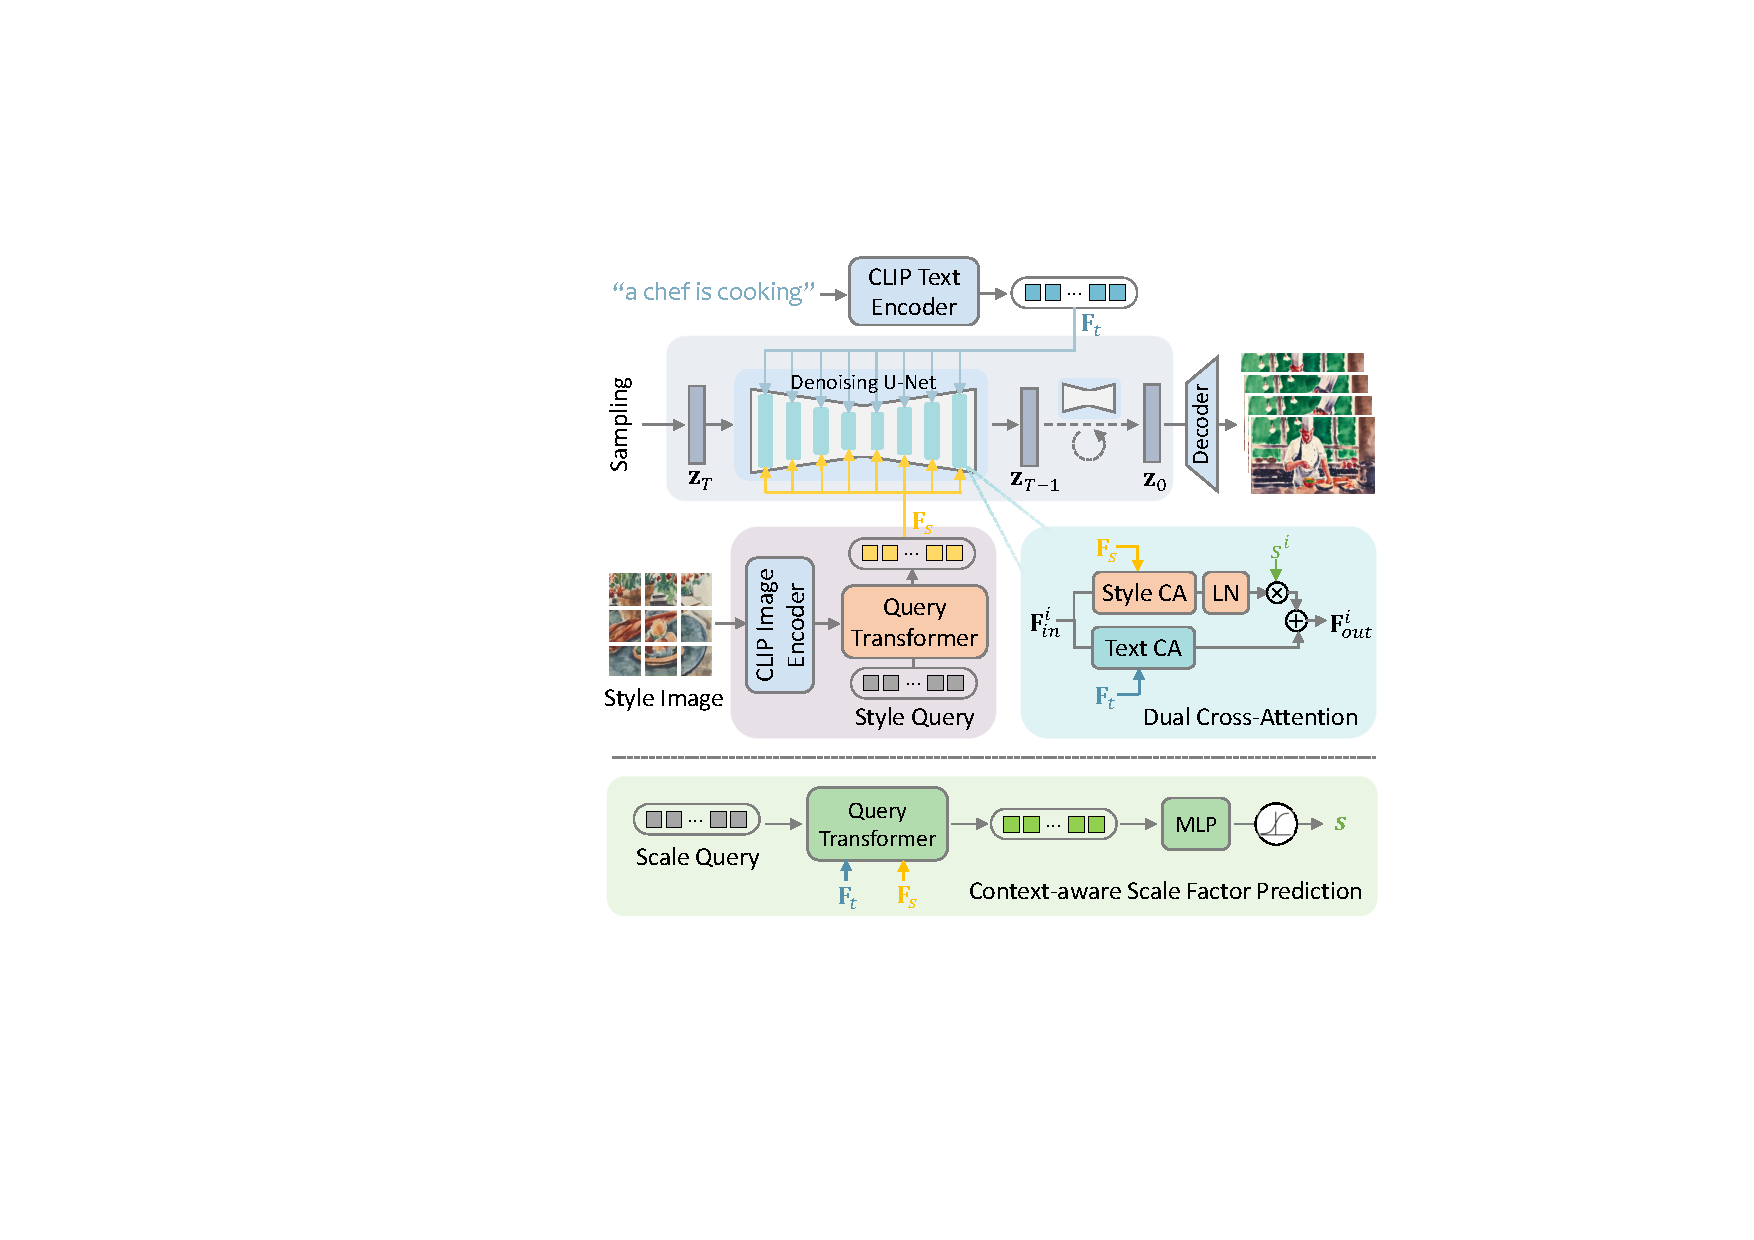
\includegraphics[width=0.95\linewidth]{figures/overview2.pdf}
    \vspace{-0.35cm}
    \caption{Overview of our proposed style adapter. It consists of three components, i.e. style feature extractor, dual cross-attention module, and context-aware scale factor predictor.}
    \label{fig:overview}
    \vspace{-1.4em}
\end{figure}


%---------------------------------
\vspace{-0.6em}
\subsection{Reference-Based Style Modulation}
\label{subsec:style_modulation}
%---------------------------------

Our style adapter serves to extract style features from the input reference image and infuse them into the backbone features of the denoising U-Net. As mainstream T2V models~\cite{chen2023videocrafter, chen2024videocrafter2, wang2023modelscope, wang2023lavie} are generally initialized from open-source T2I Models and trained with image and video datasets in a joint strategy, they support not only text-to-video generation but also retain the capacity for text-to-image generation. To overcome the scarcity of stylized videos, we propose to train the style adapter based on a pre-trained T2V model (i.e. VideoCrafter~\cite{chen2023videocrafter}) for stylized image generation under the supervision of stylistic images.

\vspace{-0.3em}
\paragraph{Content-Style Decoupled Data Augmentation.}
\label{sec:data_aug}
We use the stylistic images from two publicly available datasets, i.e. WikiArt~\cite{phillips2011wiki} and a subset of Laion-Aesthetics~\cite{schuhmann2022laion} (aesthetics score above 6.5). In the original image-caption pairs, we observe that the captions generally contain both content and style descriptions, and some of them do not match the image content well. To promote the content-style decoupling, we use BLIP\nobreakdash-2~\cite{li2023blip2} to regenerate captions for the images and remove certain forms of style description (e.g., \textit{a painting of}) with regular expressions.
In addition, as an image contains both style and content information, it is necessary to construct a decoupling supervision strategy to guarantee the extracted style feature free of content features. Although a stylistic image may contain different local style patterns~\cite{park2019arbitrary, huo2021manifold, chen2023tssat}, we regard that a large crop of an image(e.g. 50\% of the image) still preserves a similar style representation with the full image.
% We regard that every local regions of a stylistic image share the same style representation, which not only reflects on texture and color theme but also on the structure and perceptual semantics. 
Based on this insight, we process each stylistic image to obtain the target image and style image through different strategies: for target image, we scale the shorter side of the image to 512 and then crop the target content from the central area; for style image, we scale the shorter side of the image to 800 and randomly crop a local patch with $512 \times 512$. This approach reduces the overlap between the style reference and generation target, while still preserving the global style semantics complete and consistent.

\vspace{-0.3em}
\paragraph{Style Embedding Extraction.}
CLIP~\cite{radford2021learning} has demonstrated remarkable capability in extracting visual features from open-domain images. To capitalize on this advantage, we employ a pre-trained CLIP image encoder as a feature extractor. Specifically, we utilize both the global semantic token and the full $256$ local tokens (i.e., from the final layer of the Transformer) since our desired style embedding should not only serve as an accurate style trigger for the T2V model, but also provide auxiliary feature references.
As image tokens encompass both style and content information, we further employ a trainable Query Transformer (Q-Former)~\cite{li2023blip2} to extract style embedding $\mathbf{F}_s$. We create $N$ learnable style query embeddings as input for the Q-Former, which interact with image features through self-attention layers.
%We define style as the synthesized information present in an image that characterizes its overall aesthetic, independent of content. It encompasses both high-level aesthetic semantic information, such as composition, artistic conception, and color scheme, as well as low-level texture information, including specific brush stokes, lines, and surface details.
Note that this is a commonly adopted architecture for visual condition extraction~\cite{li2023blip2, shi2023instancebooth,ye2023ipadapter, xing2023dynamicrafter}. But it is the style-content fusion mechanism that makes our proposed design novel and insightful for style modulation, as detailed below.

\begin{figure}[t]
    \centering
    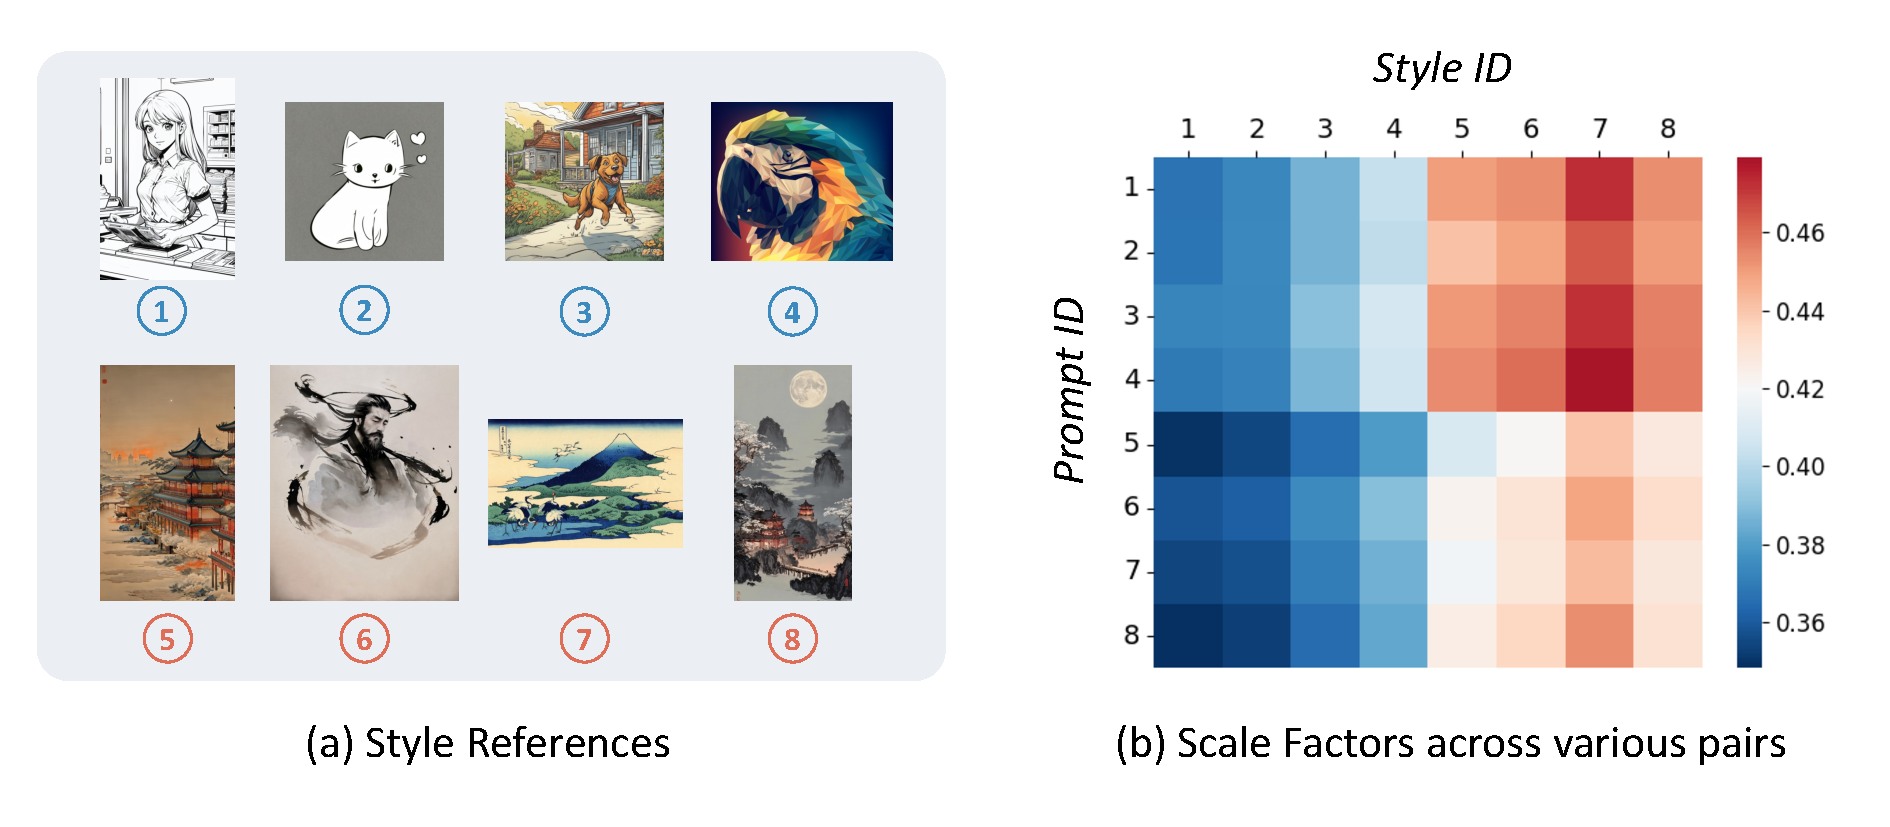
\includegraphics[width=\linewidth]{figures/scale_factor_viz.pdf}
    \vspace{-1.0cm}
    \caption{Illustration of content-style fusion scale factors across multiple input pairs. Four short prompts(less than 5 words) with prompt id $\in [1, 4]$ and four long prompts(more than 8 words) with prompt id $\in [5, 8]$ are randomly selected. Results indicate that shorter prompts and images with richer style-semantics tend to have relatively higher scale factors.} 
    \label{fig:scale_factor_viz}
    \vspace{-0.35cm}
\end{figure}

\paragraph{Adaptive Style-Content Fusion.}
\label{sec:fusion}
With the extracted style embedding, there are two ways to combine the style and text conditions, including (i) \textit{attach-to-text}~\cite{composer,gligen,ramesh2022hierarchical}: attach the style embedding to the text embedding and then interact with the backbone feature via the originally text-based cross-attention as a whole; (ii) \textit{dual cross-attention}~\cite{wei2023elite,ye2023ipadapter}: adding a new cross-attention module for the style embedding and then fuse the text-conditioned feature and style-conditioned feature.
According to our experiment (see Sec.~\ref{subsec:ablation}), solution (ii) surpasses solution (i) in disentangling the roles of text and style conditions, therefore we have adopted it as our final solution. The formula can be written as:
\vspace{-0.3em}
\begin{equation}
    \mathbf{F}_{out}^{i} = \text{TCA}(\mathbf{F}_{in}^i, \mathbf{F}_t) + s^i * \text{LN}(\text{SCA}(\mathbf{F}_{in}^i, \mathbf{F}_s)),
\end{equation}
where $\mathbf{F}_{in}^i$ denotes the backbone feature of layer $i$, LN denotes layer normalization, and TCA and SCA denote text-based cross attention and style-based cross attention respectively. $s^i$ is a scale factor learned by a context-aware scale factor prediction network, to balance the magnitudes of text-based feature and style-based feature.
The motivation is that different stylistic genres may have different emphasis on content expression. For example, the abstract styles tend to diminish the concreteness of the content, while realism styles tend to highlight the accuracy and specificity of the content. So, we propose a context-aware scale factor prediction network to predict fusion scale factors according to the input contexts.
Specifically, we create a learnable factor query, it interacts with textual features $\mathbf{F}_t$ and style features $\mathbf{F}_s$ to generate scale features via a Q-Former and then project it into layer-wise scale factors $\mathbf{s} \in \mathbb{R}^{16}$.
Figure~\ref{fig:scale_factor_viz} illustrates the learned scale factors across multiple contexts. It shows that the adaptive scale factors have a strong correlation with style genres while also depending on the text prompts. Style references with rich style-semantics(i.e., ukiyo-e style) typically yield higher scale factors to emphasize style; while complex prompts tend to produce lower scale factors to enhance content control.  This is consistent with our hypothesis to motivate our design.


%---------------------------------
\vspace{-0.5em}
\subsection{Temporal Adaptation to Stylized Features}
\label{subsec:temp_adaptation}
%---------------------------------

Given a pre-trained T2V model, the style adapter trained on image dataset works well for stylized image generation. However, it still struggles to generate satisfactory stylized videos, which is vulnerable to temporal jittering and visual artifacts.
The possible causes are that the cross-frame operations, i.e. temporal self-attention, do not involve in the process of stylized image generation, and thus induce incompatible issues. So, it is necessary to finetune the temporal self-attention with the style adapter incorporated.
Following the practice of T2V image and video joint training, the finetuning is performed on the mixed datasets of stylistic images and photorealistic videos. This is an adaptation training of temporal blocks while the other modules remain frozen, and the model converges efficiently.

\vspace{-0.5em}
\paragraph{Classifier-Free Guidance for Multiple Conditions.}
Unlike T2I models, video models exhibit a higher sensitivity to style guidance due to their limited stylized generation capabilities. Using a unified $\lambda$ for both style and context guidance may lead to undesirable generation results. Regarding this, we adopt a more flexible mechanism for multiple conditions classifier-free guidance. Building upon the vanilla text-guided classifier-free guidance, which controls context alignment by contrasting textual-conditioned distribution $\epsilon(z_t, c_t)$ with unconditional distribution $\epsilon(z_t, \varnothing)$, we introduce the style guidance with $\lambda_s$ by emphasizing the difference between the text-style-guided distribution $\epsilon(z_t, c_t, c_s)$ and the text-guided distribution $\epsilon(z_t, c_t)$. The complete formulation is as below:
\begin{equation}
    \begin{aligned}
        \hat{\epsilon}(z_t, c_t, c_s) = \epsilon(z_t, \varnothing) &+ \lambda_s(\epsilon(z_t, c_t, c_s) - \epsilon(z_t, c_t)) \\
        &+ \lambda_t(\epsilon(z_t, c_t) - \epsilon(z_t, \varnothing)),
    \end{aligned}
\end{equation}
where $c_t$ and $c_s$ denote textual and style condition respectively. $\varnothing$ denotes using no text or style conditions.
In our experiment, we follow the recommended configuration of text guidance in VideoCrafter~\cite{chen2023videocrafter}, setting $\lambda_t = 15.0$, while the style guidance is configured with $\lambda_s = 7.5$ empirically. Similarly, we set $\lambda_t = 7.5$ and $\lambda_s = 5.0$ for style-guided image generation.





